\documentclass{article}
\usepackage[utf8]{inputenc}
\usepackage{amsmath}
\usepackage{pgfplots}
\title{Robotics prereq math}
\author{Intro to Robotics}
\date{}

\begin{document}

\maketitle

%notes from 1-3
\section{List of topics to know}
1. Matrix addition and multiplication\\
2. Reduced Row echelon form to get inverse of a matrix and solve for x\\
3. Determinants\\ 
4. cross products\\
6. dot products\\
4. Transpose \\
5. Eigenvalues(we will see later in the semester)\\

\section{How to look at matrices}
\textbf{Column Picture}\\
$Ax=b$, Let $A = \begin{bmatrix}v_1 &v_2\end{bmatrix}$ where $v_1, \text{and } v_2$ are column vectors. The column picture is posing the problem $x_1v_1+x_2v_2=b$, aka how do we add the column vectors scaled by the entries in x, to get b.\\\\
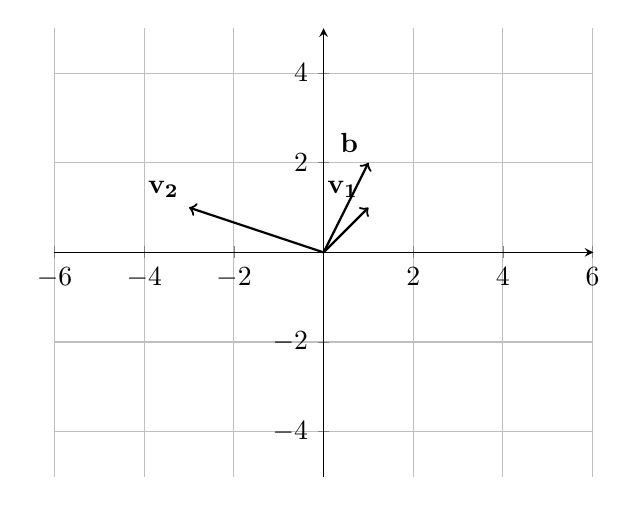
\begin{tikzpicture}
\begin{axis}[axis lines=middle, xmin=-5, xmax=5, ymin=-5,ymax=5,axis equal,grid=both]
\addplot [->, thick,  black] coordinates { (0,0) (1,1)}node[above left]{$\mathbf{v_1}$};
\addplot [->, thick,  black] coordinates { (0,0) (-3,1)}node[above left]{$\mathbf{v_2}$};
\addplot [->, thick,  black] coordinates { (0,0) (1,2)}node[above left]{$\mathbf{b}$};
\end{axis}
\end{tikzpicture}
\newpage
\textbf{Row picture}\\
$Ax=b$, Consider the rows of A as being equations such that row n is $a_{n1}x_1+a_{n2}x_2+...+a_{nm}x_m=b_n$, this row gives us an m-1 size plane that are all the possible solutions to the equation in m dimension. All the rows live in some n dimensional space and their point of intersection is the vector $x$.\\\\
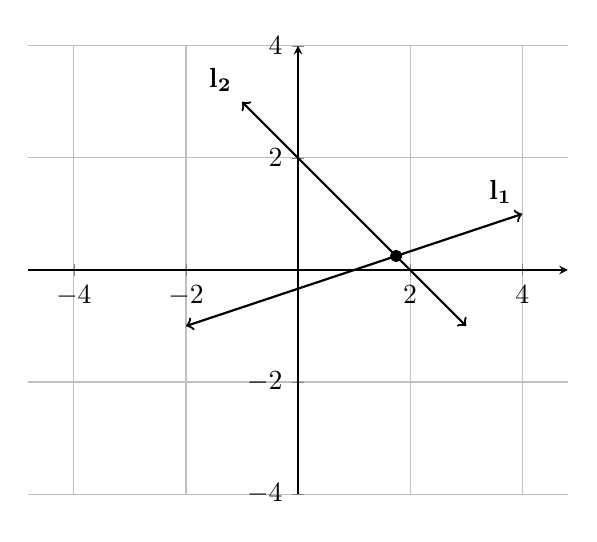
\begin{tikzpicture}
\begin{axis}[axis lines=middle, xmin=-4, xmax=4, ymin=-4,ymax=4,axis equal,grid=both]
\addplot [<->, thick,  black] coordinates { (-2,-1) (4,1)}node[above left]{$\mathbf{l_1}$};
\addplot [<->, thick,  black] coordinates { (3,-1) (-1,3)}node[above left]{$\mathbf{l_2}$};
\addplot [only marks] table {
1.75 .25
};
\end{axis}
\end{tikzpicture} \\\\
\section{Matrix Addition}
For matrix addition just add up the corresponding entries, for example: \\
$\begin{bmatrix}
1 & 2 & 3 \\
4 & 5 & 6 \\
7 & 8 & 9
\end{bmatrix}+\begin{bmatrix}
1 & -1 & 1 \\
0 & 2 & 2 \\
1 & -2 & 0
\end{bmatrix}=
\begin{bmatrix}
2 & 1 & 4 \\
4 & 7 & 8 \\
8 & 6 & 9
\end{bmatrix}$\\\\
If the dimensions of the matrices do not match, then matrix addition is not possible. For example:\\
$\begin{bmatrix}
1 & 2 & 3 \\
4 & 5 & 6 \\
\end{bmatrix}+\begin{bmatrix}
1 & -1  \\
0 & 2 \\
1 & -2
\end{bmatrix}=$ NOT POSSIBLE\\\\
Geometrically, the column vectors are being combined. Take a look at regular matrix addition for $\begin{bmatrix}1 \\ 3 \end{bmatrix} + \begin{bmatrix}2 \\ 2 \end{bmatrix}=\begin{bmatrix}3 \\ 5 \end{bmatrix}$.\\\\
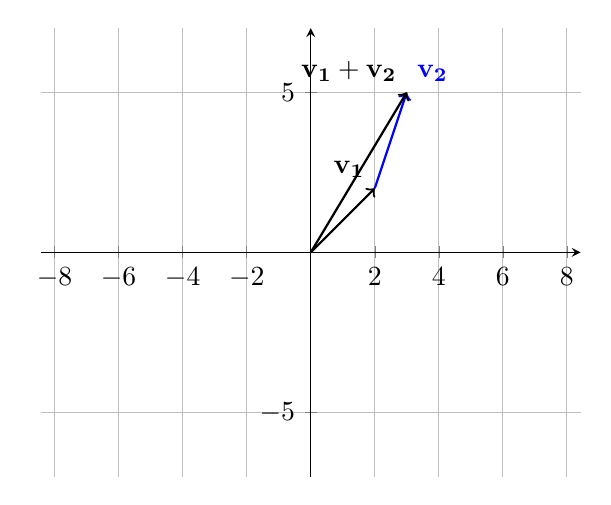
\begin{tikzpicture}
\begin{axis}[axis lines=middle, xmin=-7, xmax=7, ymin=-7,ymax=7,axis equal,grid=both]
\addplot [->, thick,  black] coordinates { (0,0) (2,2)}node[above left]{$\mathbf{v_1}$};
\addplot [->, thick,  blue] coordinates { (2,2) (3,5)}node[above right]{$\mathbf{v_2}$};
\addplot [->, thick,  black] coordinates { (0,0) (3,5)}node[above left]{$\mathbf{v_1+v_2}$};
\end{axis}
\end{tikzpicture} \\\\

\section{Matrix Multiplication}
Matrix multiplication is at the root of linear algebra, just look at the main problem $Ax=b$ above, this is a matrix multiplication. Both column picture and row picture are a valid geometric interpretation of matrix multiplication.\\
\textbf{Matrix multiplication rule}\\
$\begin{bmatrix}
a_{11} & a_{12} & a_{13} \\
a_{21} & a_{22} & a_{23} \\
a_{31} & a_{32} & a_{33}
\end{bmatrix}\begin{bmatrix}
x_{1}  \\
x_{2}  \\
x_{3} 
\end{bmatrix}=
\begin{bmatrix}
a_{11}x_1 + a_{12}x_2 + a_{13}x_3 \\
a_{21}x_1 + a_{22}x_2 + a_{23}x_3 \\
a_{31}x_1 + a_{32}x_2 + a_{33}x_3
\end{bmatrix}$\\\\
\textbf{Examples:}\\
$\begin{bmatrix}
1 & 0 & 2 \\
-3 & 5 & 9 \\
1 & -2 & 7
\end{bmatrix}\begin{bmatrix}
1  \\
2  \\
-8 
\end{bmatrix}=
\begin{bmatrix}
-15 \\
-65 \\
-59
\end{bmatrix}$\\\\
$\begin{bmatrix}
1 & 0 & 2 \\
-3 & 5 & 9 \\
1 & -2 & 7
\end{bmatrix}\begin{bmatrix}
1 &  \textcolor{red}{0}\\
2 & \textcolor{red}{1}\\
-8 & \textcolor{red}{2}
\end{bmatrix}=
\begin{bmatrix}
-15 & \textcolor{red}{4}\\
-65 & \textcolor{red}{23}\\
-59 & \textcolor{red}{12}
\end{bmatrix}$\\\\
\textbf{Three things to note:}\\
\textbf{1.)} Notice that adding a column to the second input matrix(labeled red), only modifies the output matrix by adding a second column to the output matrix(labeled red). This new column gets multiplied by the first input matrix(independent of the first column in the second matrix) to produce the second column in the output matrix using the multiplication rule mentioned above.In general, This is how matrix multiplication works for matrices of all sizes(assuming they're compatible for the operation).\\\\
\textbf{2.)} In order for matrix multiplication to be compatible the the number of columns of the first matrix must match the number of rows of the second matrix. For example:\\
$\begin{bmatrix}
1 & -2 & 3 & -4\\
-5 & 6 & -7 & 8 \\
9 & -10 & 11 & -12 \\
-13 & 14 & -15 & 16
\end{bmatrix}\begin{bmatrix}
1 & 3 & 0\\
2 & 4 & -1\\
-1 & -2 & 1\\
1 & 2 & -1
\end{bmatrix}=
\begin{bmatrix}
-10 & -19 & 9\\
22 & 39 & -21\\
-34 & -59 & 33\\
46 & 79 & -45
\end{bmatrix}$\\
These are compatible because the dimension (rows, columns) are (4,4) for the first matrix and (4,3) for the second matrix, notice that the columns of the first matrix match the rows of the second matrix. However if we flip these matrices we get:
$\begin{bmatrix}
1 & 3 & 0\\
2 & 4 & -1\\
-1 & -2 & 1\\
1 & 2 & -1
\end{bmatrix}\begin{bmatrix}
1 & -2 & 3 & -4\\
-5 & 6 & -7 & 8 \\
9 & -10 & 11 & -12 \\
-13 & 14 & -15 & 16
\end{bmatrix}=$ NOT COMPATIBLE\\\\
Now the first matrix dimensions are (4,3) and the second matrix dimensions are (4,4). The columns of the first matrix no longer match the rows of the second matrix, thus making the matrices not compatible for multiplication.\\
\textbf{3.)} Matrix multiplication is associative but not commutative. In general:\\
$(AB)C =A(BC)$ \\
$AB \neq BA$ 


\section{Rref and inverses}
Rref stands for row reduced echelon form and it is an algorithm used for reducing a matrix into the identity matrix(if it is non-singular). The identity matrix is a square matrix with 1's along the diagonal and 0's everywhere else.\\
Identity matrix examples:$\begin{bmatrix}
1 & 0 \\
0 & 1
\end{bmatrix}, \begin{bmatrix}
1 & 0 & 0\\
0 & 1 & 0\\
0 & 0 & 1 
\end{bmatrix}
, \begin{bmatrix}
1 & 0 & 0 & 0\\
0 & 1 & 0 & 0\\
0 & 0 & 1 & 0\\
0 & 0 & 0 & 1
\end{bmatrix}$(All denoted by I)\\\\
If the end result of rref is not the identity matrix, then we know that our matrix is singular, which means it has determinant equal to zero. The rules for performing rref are as follows:\\
\textbf{1. } You can swap rows(not columns)\\
\textbf{2. } You can multiply/divide a row by any scalar\\
\textbf{3. } You can add/subtract one row from another\\
\textbf{Example: }
$\left[
\begin{array}{ccc|c}
0 & 2 & -1 & 4  \\
3 & -2 & 1 & 3  \\
3 & 2 & 1 & -1  \\
\end{array}
\right]
\rightarrow
\left[
\begin{array}{ccc|c}
3 & -2 & 1 & 3  \\
0 & 2 & -1 & 4  \\
3 & 2 & 1 & -1  \\
\end{array}
\right]
\rightarrow
\left[
\begin{array}{ccc|c}
3 & -2 & 1 & 3  \\
0 & 2 & -1 & 4  \\
0 & 4 & 0 & -4  \\
\end{array}
\right]
\rightarrow
\left[
\begin{array}{ccc|c}
3 & -2 & 1 & 3  \\
0 & 4 & 0 & -4  \\
0 & 2 & -1 & 4  \\
\end{array}
\right]
\rightarrow
\left[
\begin{array}{ccc|c}
3 & -2 & 1 & 3  \\
0 & 4 & 0 & -4  \\
0 & 0 & 1 & -6  \\
\end{array}
\right]
\rightarrow
\left[
\begin{array}{ccc|c}
3 & -2 & 1 & 3  \\
0 & 1 & 0 & -1  \\
0 & 0 & 1 & -6  \\
\end{array}
\right]
\rightarrow
\left[
\begin{array}{ccc|c}
3 & 0 & 1 & 1  \\
0 & 1 & 0 & -1  \\
0 & 0 & 1 & -6  \\
\end{array}
\right]
\rightarrow
\left[
\begin{array}{ccc|c}
3 & 0 & 0 & 7  \\
0 & 1 & 0 & -1  \\
0 & 0 & 1 & -6  \\
\end{array}
\right]
\rightarrow
\left[
\begin{array}{ccc|c}
1 & 0 & 0 & \frac{7}{3}  \\
0 & 1 & 0 & -1  \\
0 & 0 & 1 & -6  \\
\end{array}
\right]$\\
\textbf{Heuristic to follow- always convert zeros below the diagonal first.}\\
\textbf{Check work, make sure matrix multiplication here works}\\\\
$\begin{bmatrix}
0 & 2 & -1  \\
3 & -2 & 1   \\
3 & 2 & 1 &  
\end{bmatrix}
\begin{bmatrix}
\frac{7}{3}  \\
-1  \\
-6 
\end{bmatrix}=
\begin{bmatrix}
4  \\
3  \\
-1 
\end{bmatrix}
$\\\\

\textbf{To get the inverse of a matrix, you must perform the rref algorithm slightly modified. Remove the output vector from the matrix and replace it with the identity matrix. Now perform rref as usual to both sides.} $AA^{-1}=A^{-1}A=I$(where I is identity matrix)\\\\
\textbf{Example: }
$\left[
\begin{array}{ccc|ccc}
1 & 2 & -1 & 1 & 0 & 0\\
2 & 1 & 2 & 0 & 1 & 0\\
-1 & 2 & 1 & 0 & 0 & 1  \\
\end{array}
\right]
\rightarrow
\left[
\begin{array}{ccc|ccc}
1 & 2 & -1 & 1 & 0 & 0\\
2 & 1 & 2 & 0 & 1 & 0\\
0 & 4 & 0 & 1 & 0 & 1  \\
\end{array}
\right]
\rightarrow
\left[
\begin{array}{ccc|ccc}
1 & 2 & -1 & 1 & 0 & 0\\
0 & -3 & 4 & -2 & 1 & 0\\
0 & 4 & 0 & -2 & 1 & 0  \\
\end{array}
\right]
\rightarrow
\left[
\begin{array}{ccc|ccc}
1 & 2 & -1 & 1 & 0 & 0\\
0 & 1 & 0 & \frac{1}{4} & 0 & \frac{1}{4}\\
0 & -3 & 4 & 1 & 0 & 1  \\
\end{array}
\right]
\rightarrow
\left[
\begin{array}{ccc|ccc}
1 & 2 & -1 & 1 & 0 & 0\\
0 & 1 & 0 & \frac{1}{4} & 0 & \frac{1}{4}\\
0 & 0 & 4 & -\frac{5}{4} & 1 & \frac{3}{4}  \\
\end{array}
\right]
\rightarrow
\left[
\begin{array}{ccc|ccc}
1 & 2 & -1 & 1 & 0 & 0\\
0 & 1 & 0 & \frac{1}{4} & 0 & \frac{1}{4}\\
0 & 0 & 1 & -\frac{5}{16} & \frac{1}{4} & \frac{3}{16}  \\
\end{array}
\right]
\rightarrow
\left[
\begin{array}{ccc|ccc}
1 & 2 & 0 & \frac{11}{16} & \frac{1}{4} & \frac{3}{16}\\
0 & 1 & 0 & \frac{1}{4} & 0 & \frac{1}{4}\\
0 & 0 & 1 & -\frac{5}{16} & \frac{1}{4} & \frac{3}{16}  \\
\end{array}
\right]
\rightarrow
\left[
\begin{array}{ccc|ccc}
1 & 0 & 0 & \frac{3}{16} & \frac{1}{4} & -\frac{5}{16}\\
0 & 1 & 0 & \frac{1}{4} & 0 & \frac{1}{4}\\
0 & 0 & 1 & -\frac{5}{16} & \frac{1}{4} & \frac{3}{16}  \\
\end{array}
\right]$\\\\
\textbf{Check work by verifying that $AA^{-1}=I$}\\
$\begin{bmatrix}
1 & 2 & -1 \\
2 & 1 & 2 \\
-1 & 2 & 1 
\end{bmatrix}
\begin{bmatrix}
\frac{1}{4} & -\frac{5}{16}\\
\frac{1}{4} & 0 & \frac{1}{4}\\
-\frac{5}{16} & \frac{1}{4} & \frac{3}{16} 
\end{bmatrix}=
\begin{bmatrix}
1 & 0 & 0 \\
0 & 1 & 0 \\
0 & 0 & 1 
\end{bmatrix}$\\\\

\section{Transpose}
The transpose of a matrix is constructed by swapping the rows of a matrix by its own columns. We will use transposes often when discussing rotation matrices. \\
\textbf{Example: }\\
$A=\begin{bmatrix}
1 & 0 & 3 & 4\\
1 & 1 & -2 & 6\\
-1 & 2 & 8 & -3\\
-1 & 7 & 1 & -5
\end{bmatrix};
A^T=\begin{bmatrix}
1 & 1 & -1 & -1\\
0 & 1 & 2 & 7\\
3 & -2 & 8 & 1\\
4 & 6 & -3 & -5
\end{bmatrix}$\\
Where $A^T$ is the transpose of A.
\newpage
\section{Determinants}
One geometric interpretation of the determinant is that it is the area of the column vectors enclosed.\\
Consider the matrix A=
$\begin{bmatrix}
1 & 2\\
2 & -1 
\end{bmatrix}$ and denote its column vectors as $v_1$ and $v_2$. Now we can enclose the column vectors by filling out the parallelogram with the blue vectors below(denoted $e_1$ and $e_2$). The area of this parallelogram is the determinant of matrix A. This extends to 3d space where the determinant is equal to the \textbf{volume} of the enclosed parallelopipe. \\
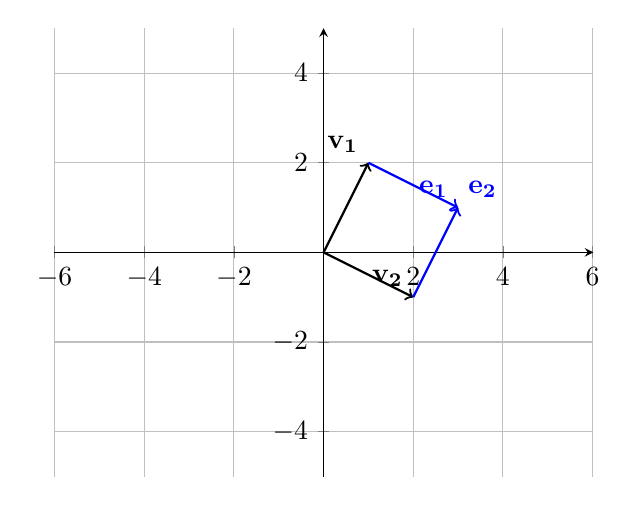
\begin{tikzpicture}
\begin{axis}[axis lines=middle, xmin=-5, xmax=5, ymin=-5,ymax=5,axis equal,grid=both]
\addplot [->, thick,  black] coordinates { (0,0) (1,2)}node[above left]{$\mathbf{v_1}$};
\addplot [->, thick,  black] coordinates { (0,0) (2,-1)}node[above left]{$\mathbf{v_2}$};
\addplot [->, thick,  blue] coordinates { (1,2) (3,1)}node[above left]{$\mathbf{e_1}$};
\addplot [->, thick,  blue] coordinates { (2,-1) (3,1)}node[above right]{$\mathbf{e_2}$};
\end{axis}
\end{tikzpicture}\\\\
Now consider a singular matrix. When a matrix is singular that implies that more than one of its column vectors are colinear. Consider the singular matrix A = 
$\begin{bmatrix}
1 & 2 \\
1 & 2
\end{bmatrix}$\\
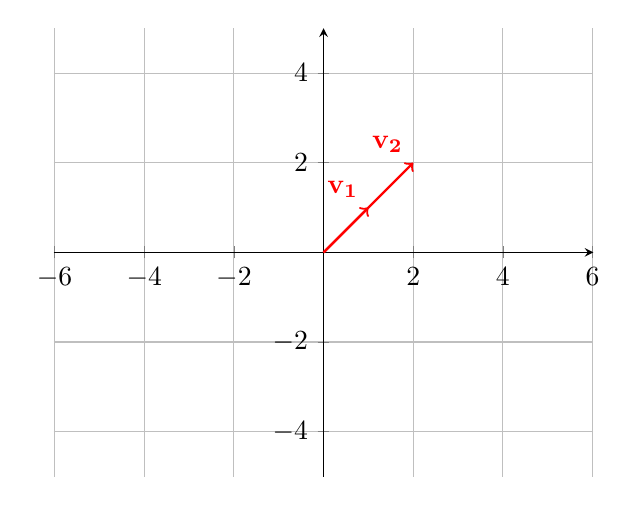
\begin{tikzpicture}
\begin{axis}[axis lines=middle, xmin=-5, xmax=5, ymin=-5,ymax=5,axis equal,grid=both]
\addplot [->, thick,  red] coordinates { (0,0) (1,1)}node[above left]{$\mathbf{v_1}$};
\addplot [->, thick,  red] coordinates { (0,0) (2,2)}node[above left]{$\mathbf{v_2}$};
\end{axis}
\end{tikzpicture}\\\\
Notice that when column vectors are colinear there is no parallelopipe to compute the area for, thus the determinant is 0.\\
\textbf{Formula for 2 by 2: }\\
$\begin{bmatrix}
a & b\\
c & d
\end{bmatrix}$ the determinant is equal to $ad-bc$\\\\
\textbf{Formula for 3 by 3: }\\
$\begin{bmatrix}
a & b & c\\
d & e & f\\
g & h & i
\end{bmatrix}$ the determinant is equal to $a(ei-fh) - b(di-fg) + c(dh-eg)$(this formula is constructed by taking the 2 by 2 determinants of the co matrix for the first row and multiplying by the elements in the first row)\\\\
\textbf{Examples: }\\
$det(
\begin{bmatrix}
1 & 2  \\
2 & -1
\end{bmatrix}) = 1*-1 - 2*2 = -5$\\
$det(
\begin{bmatrix}
3 & -2 & 1  \\
0 & 2 & -1   \\
3 & 2 & 1   
\end{bmatrix}) = 3(2*1- -1*2)- -2(0*1- -1*3) + 1(0*2-2*3) = 12 - -6 + -6 = 12$

\section{Dot product}
The dot product is a method for multiplying two vectors, it is defined as\\ $\mathbf{v_1 \cdot v_2 = v_{1}^T v_{2}}$.\\\\ 
\textbf{Example:} \\
$\begin{bmatrix}
4 \\
-1 \\
3 
\end{bmatrix} \cdot
\begin{bmatrix}
1 \\
2 \\
3 
\end{bmatrix} =
\begin{bmatrix}
4 & -1 & 3 
\end{bmatrix} 
\begin{bmatrix}
1 \\
2 \\
3 
\end{bmatrix}= 4*1 + (-1*2) + 3*3 = 11
$(since the dot product is not equal to zero we know that the vectors are not perpendicular)\\\\\\
Another definition of the dot product is that $\mathbf{v_1 \cdot v_2 = |v_{1}|| v_{2}|cos(\theta)}$\\ where theta is the angle between vectors $v_1$ and $v_2$;\\ and $|v_i|= \sqrt{v_{i,1}^2+v_{i,2}^2+ \dots + v_{i,n-1}^2+v_{i,n}^2}$(magnitude of $v_i$ where $v_i$ is a (n x 1) vector).\\
This definition is useful for solving the angles between vectors. From this definition we can infer that if two vectors are perpendicular then there dot product is 0. This is because if two vectors are perpendicular then the angle between them is 90 degrees. the cosine of 90 degrees is always 0, so the cosine term in this definition zeros out the whole dot product. \\\\
\textbf{Example:} \\
Find the angle between 
$v_1 = \begin{bmatrix}
3.48 \\
2
\end{bmatrix}$ and 
$v_2 = \begin{bmatrix}
-2.61 \\
1.5
\end{bmatrix}$\\\\
consider the equation $\frac{v_1 \cdot v_2}{|v_{1}|| v_{2}|} = cos(\theta)$\\
first compute dot product:
$\begin{bmatrix}
3.48 \\
2
\end{bmatrix} \cdot
\begin{bmatrix}
-2.61 \\
1.5
\end{bmatrix}=3.48*-2.61 + 2*1.5= -6.08$\\
Then compute length of $v_1$ and $v_2$: 
$|v_1|= \sqrt{3.48^2+2^2}=\sqrt{14.11}=3.76$,\\ $|v_2|= \sqrt{-2.61^2+1.5^2}=\sqrt{6.81+2.25}=\sqrt{9.06}=3$\\
alltogether: $cos(\theta) = \frac{v_1 \cdot v_2}{|v_{1}|| v_{2}|}=\frac{-6.08}{3.76*3}=-.54$\\
Now to get theta, when we have $cos(\theta)=.54$ we just have to use the function $arccos(cos(\theta))=arccos(-.54)\approx120^\circ $\\\\
Now let us consider the case when we are given two perpendicular vectors. 
$v_1 = \begin{bmatrix}
5 \\
-3
\end{bmatrix}$ and 
$v_2 = \begin{bmatrix}
3 \\
5
\end{bmatrix}$\\\\
Notice that on the left hand side of the equation the dot product is equal to $v_1 \cdot v_2 = 5*3 + -3*5 = 0$,
and on the right hand side we have $|v_{1}|| v_{2}|cos(\theta)$ since we know that $\theta=90^\circ$ and $cos(90^\circ)=0$
thus, $|v_{1}|| v_{2}|cos(90^\circ)=0$. 
\section{Cross product}
$v_1 \times v_2 = |v_1||v_2|sin(\theta)n$ where $n$ is the unit normal vector of the plane generated by $v_1$ and $v_2$. In other words, $n$ is a vector such that $|n|=1$ and $n$ is perpendicular to $v_1$ and $v_2$.\\\\
\textbf{Example: }\\
Given $v_1= \begin{bmatrix}
1 \\
-2 \\
1
\end{bmatrix}$ and 
$v_2= \begin{bmatrix}
2 \\
1 \\
0
\end{bmatrix}$ compute the cross product.\\\\
In order to compute the cross product we must create a matrix of the form: 
$\begin{bmatrix}
i & j & k \\
 & v_1^T & \\
 & v_2^T &
\end{bmatrix}$\\\\ 
For our problem that gives us: 
$\begin{bmatrix}
i & j & k \\
1 & -2 & 1\\
2 & 1 & 0
\end{bmatrix}$\\
Now we try to solve for the determinant of this matrix with the formula(get formula from section determinants): 
$i(-2*0 - 1*1) - j(1*0-1*2) + k(1*1-(-2*2))$ this gives us: $-1i + 2j + 5k$. The coefficient to the variables $i,j, k $ are placed in a vector, such that:\\
$\begin{bmatrix}
i (coefficient)\\
j (coefficient)\\
k (coefficient)
\end{bmatrix}$\\\\
Giving us $v_1 \times v_2 = \begin{bmatrix}
-1 \\
2 \\
5
\end{bmatrix}$
\\
\textbf{everything below is rounded to two places}\\
compute for n by dividing sizes $v_1 \times v_2$ by $|v_1 \times v_2|$.\\
$|v_1 \times v_2|=\sqrt{-1^2 + 2^2 + 5^2}=\sqrt{30}=5.48$\\\\
$n=\frac{v_1 \times v_2}{|v_1 \times v_2|}=\frac{\begin{bmatrix}
-1 \\
2 \\
5
\end{bmatrix}}{5.48} = \begin{bmatrix}
-.18 \\
.36 \\
.91
\end{bmatrix}$ \\\\
Now using the dot product we will check that $v_1$ is perpendicular to $n$ and that $v_2$ is perpendicular to $n.$\\
$v_1 \cdot n = \begin{bmatrix}
1 \\
-2\\
1
\end{bmatrix} \cdot 
\begin{bmatrix}
-.18 \\
.36 \\
.91
\end{bmatrix}= 1*-.18+ -2*.36 + 1*.91= -.18+ -.72 + .91 \approx 0$ \\
$v_1 \cdot n = \begin{bmatrix}
2 \\
1\\
0
\end{bmatrix} \cdot 
\begin{bmatrix}
-.18 \\
.36 \\
.91
\end{bmatrix}= 2*-.18+ 1*.36 + 0*.91= -.36 + .36 = 0$
\\ The slight errors above are due to rounding issues(I rounded to two places for the unit normal vector).\\\\
\begin{tikzpicture}
\begin{axis}[axis lines=middle, xmin=-3, xmax=3, ymin=-3,ymax=3, zmin=-3, zmax=3,axis equal,grid=both, scale=2]
\addplot3[->, thick,  black] coordinates { (0,0,0) (1,-2,1)}node[above left]{$\mathbf{v_1}$};
\addplot3[->, thick,  black] coordinates { (0,0,0) (2,1,0)}node[above left]{$\mathbf{v_2}$};
\addplot3[->, thick,  blue] coordinates { (0,0,0) (-1,2,5)}node[above left]{$\mathbf{v_1 \times v_2}$};
\addplot3[->, thick,  red] coordinates { (0,0,0) (-.18,.36,.91)}node[above left]{$\mathbf{n}$};
\end{axis}
\end{tikzpicture}

\end{document}
